\documentclass[tikz,border=2pt,11pt]{standalone}
\usetikzlibrary{arrows.meta}
\usetikzlibrary{calc}
\usetikzlibrary{positioning}
\usepackage{amsmath}
\usepackage{amssymb}
\usepackage{mathrsfs}
\usepackage{xcolor}
\usepackage{tikz}
\newcommand{\C}{\mathbb C}
\newcommand{\R}{\mathbb R}
\newcommand{\Z}{\mathbb Z}
\newcommand{\N}{\mathbb N}
\newcommand{\E}{\mathbb E}
\newcommand{\Prob}{\mathbb P}
\DeclareMathOperator{\diam}{diam}
\DeclareMathOperator{\tr}{tr}
\DeclareMathOperator{\supp}{supp}
\DeclareMathOperator{\dist}{dist}
\DeclareMathOperator{\Var}{Var}
\begin{document}
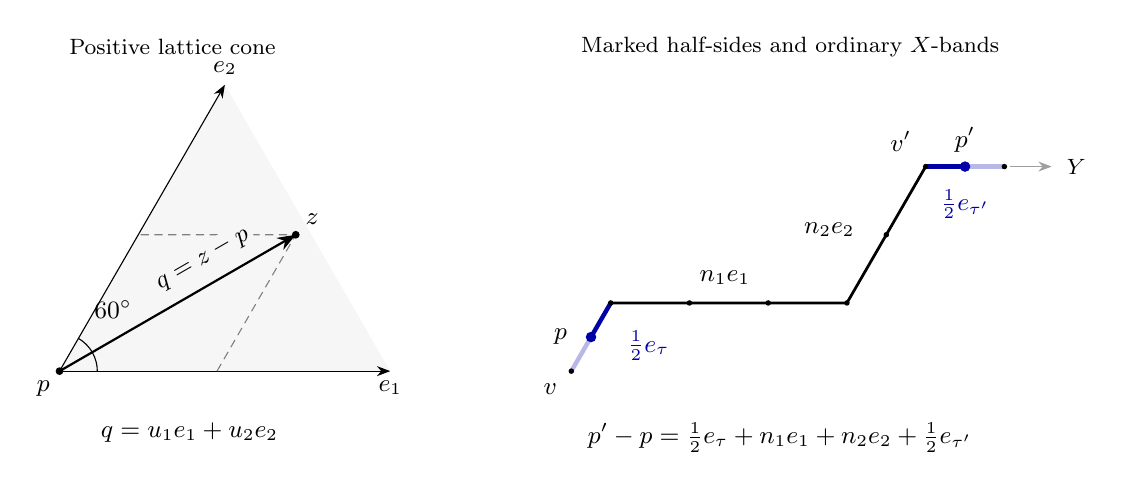
\begin{tikzpicture}[x=1cm,y=1cm,font=\small,>=Stealth,
  row/.style={line width=1pt,line join=round},
  marker/.style={line width=1.6pt,blue!65!black}]
 \begin{scope}
  \coordinate (p) at (0,0);
  \coordinate (q) at (3,1.732);
  \fill[gray!7] (p)--(4.20,0)--(2.10,3.637)--cycle;
  \draw[->] (p)--(4.20,0) node[below] {$e_1$};
  \draw[->] (p)--(2.10,3.637) node[above] {$e_2$};
  \draw[densely dashed,gray] (2,0)--(q)--(1,1.732);
  \draw[->,line width=.8pt] (p)--(q);
  \fill (p) circle (1.4pt) node[below left] {$p$};
  \fill (q) circle (1.4pt) node[above right] {$z$};
  \draw (.48,0) arc (0:60:.48);
  \node at (.68,.78) {$60^\circ$};
  \node[rotate=30,fill=gray!7,inner sep=1.5pt] at (1.82,1.42) {$q=z-p$};
  \node[anchor=west,font=\footnotesize] at (0,4.12) {Positive lattice cone};
  \node[anchor=north] at (1.65,-.53) {$q=u_1e_1+u_2e_2$};
 \end{scope}
 \begin{scope}[xshift=6.5cm]
  \coordinate (v) at (0,0);
  \coordinate (p) at (.25,.433);
  \coordinate (w) at (.5,.866);
  \coordinate (vp) at (4.5,2.598);
  \coordinate (pp) at (5,2.598);
  \coordinate (end) at (5.5,2.598);
  \draw[marker,opacity=.28] (v)--(p);
  \draw[marker] (p)--(w);
  \draw[row] (w)--(3.5,.866)--(vp);
  \draw[marker] (vp)--(pp);
  \draw[marker,opacity=.28] (pp)--(end);
  \foreach \x/\y in {0/0,.5/.866,1.5/.866,2.5/.866,3.5/.866,4/1.732,4.5/2.598,5.5/2.598}
    \fill (\x,\y) circle (1pt);
  \fill[blue!65!black] (p) circle (1.9pt);
  \fill[blue!65!black] (pp) circle (1.9pt);
  \node[anchor=east] at (.07,.44) {$p$};
  \node[anchor=south] at (5,2.66) {$p'$};
  \node[anchor=north east] at (-.06,-.04) {$v$};
  \node[anchor=south east] at (4.44,2.67) {$v'$};
  \node[anchor=south] at (1.95,.98) {$n_1e_1$};
  \node[anchor=east] at (3.72,1.80) {$n_2e_2$};
  \node[anchor=west,text=blue!65!black] at (.59,.32) {$\tfrac12e_\tau$};
  \node[text=blue!65!black] at (5.0,2.12) {$\tfrac12e_{\tau'}$};
  \draw[->,gray!75] (5.57,2.598)--(6.10,2.598);
  \node[anchor=west,font=\footnotesize] at (6.17,2.598) {$Y$};
  \node[anchor=west,font=\footnotesize] at (0,4.12) {Marked half-sides and ordinary $X$-bands};
  \node[anchor=north,align=center] at (2.65,-.53)
    {$p'-p=\tfrac12e_\tau+n_1e_1+n_2e_2+\tfrac12e_{\tau'}$};
 \end{scope}
\end{tikzpicture}
\end{document}
